   
\documentclass[11pt]{article}
\usepackage{amsmath,amsthm,verbatim,amssymb,amsfonts,amscd, graphicx}
\usepackage{graphicx}
\usepackage{float}
\usepackage{url}
\graphicspath{{./times/}}
\topmargin0.0cm
\headheight0.0cm
\headsep0.0cm
\oddsidemargin0.0cm
\textheight23.0cm
\textwidth16.5cm
\footskip1.0cm

\begin{document}
\title{CS 5220\\ Project 1 - Matrix Multiplication}
\author{Sheroze Sheriffdeen(mss385)\\ Weici Hu(wh343)\\  Qinyu Wang(qw78)}
\maketitle

\section{Introduction}
\textbf{D}ouble Precision \textbf{GE}neral \textbf{M}atrix \textbf{M}ultiplication (DGEMM) is an important operation in problems that arise in scientific and engineering computing applications. Our DGEMM function takes 2 dense square double precision matrices $A$ and $B$ stored in column major format and returns,
	\begin{equation} 
		A \times B = C
	\end{equation}
	
	where '$\times$' represents matrix multiplication. This document describes an optimized DGEMM implementation and details the design decisions used to improve performance. 

\section{Implementation Overview}
\begin{figure}[H]
\centering
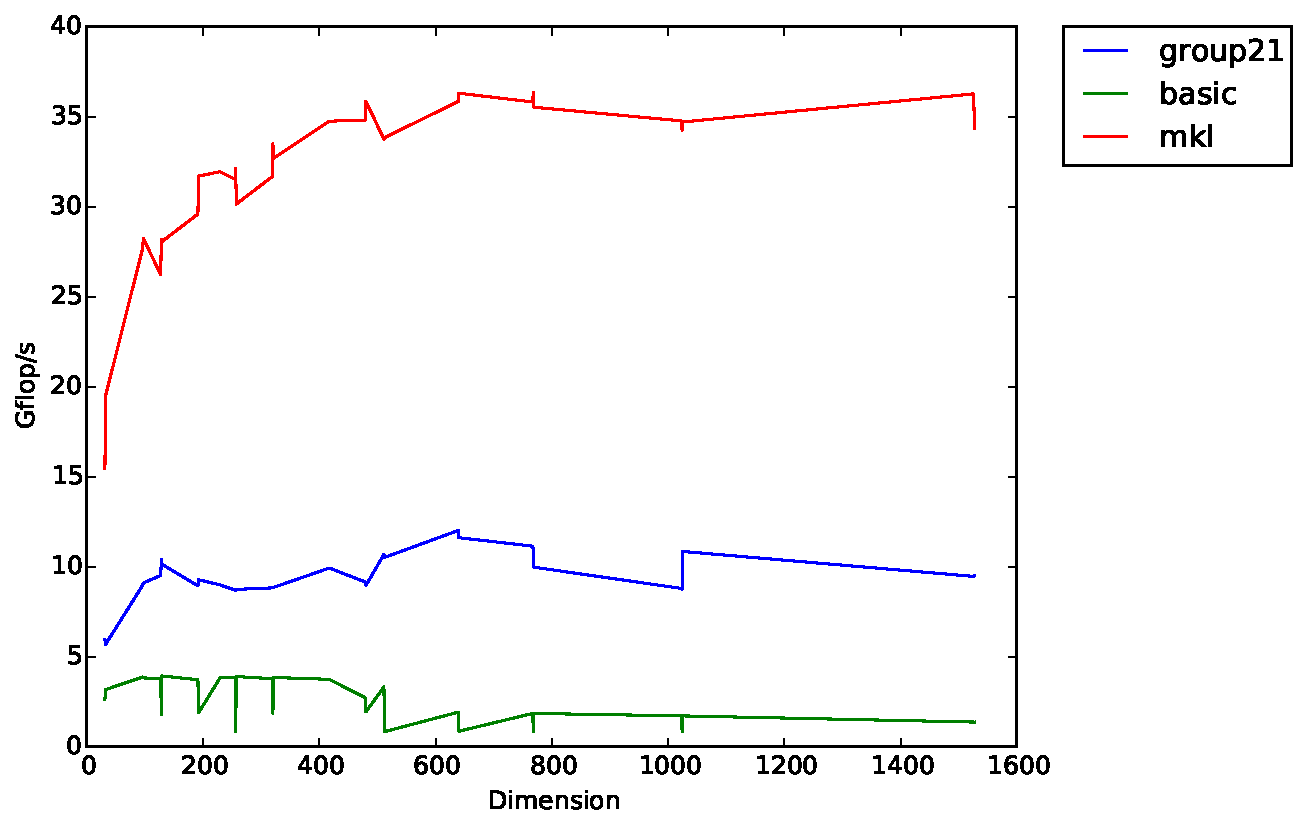
\includegraphics[scale=0.6]{growth_final.pdf}
\caption{Performance comparison: Intel MKL vs our implementation vs the naive implementation}
\end{figure}
\newpage
Our DGEMM implementation has 2 distinct modes of operation: hybrid between tight loops and blocking. On square matrices with leading dimension $<$ \texttt{BLOCK\_THRESHOLD}, our DGEMM uses tight loops with copy optimization. (Section \ref{sec:copy_opt}). \texttt{BLOCK\_THRESHOLD} was picked to be 400 elements. After this threshold, the blocked approach performs better. \\

On matrices with the leading dimension $>$ \texttt{BLOCK\_THRESHOLD}, we switch to a blocked matrix multiplication. Each block has $32 \times 32$ elements. Prior to blocking the matrices, we perform copy optimization on $A$ (transpose and copy over data to a 64 byte aligned block obtained by Intel's \texttt{mm\_malloc}). Furthermore, we also copy over data from $B$ to an aligned block and also create an aligned storage area for $C$. The newly allocation dynamic memory uses zero padding so that all block multiplication is similar. (Section \ref{sec:block}) \\

On each block, we perform the naive matrix multiplication using tight loops. To make use of the aligned data, we provide hints to the compiler by adding the $\texttt{\_\_assume\_aligned}$ clause prior to the loop using the matrix data. \cite{vectorization} Furthermore, since $A$ is transposed due to copy optimization, the innermost loop of the block multiplication is performed with stride 1. \\

\begin{figure}[H]
\centering
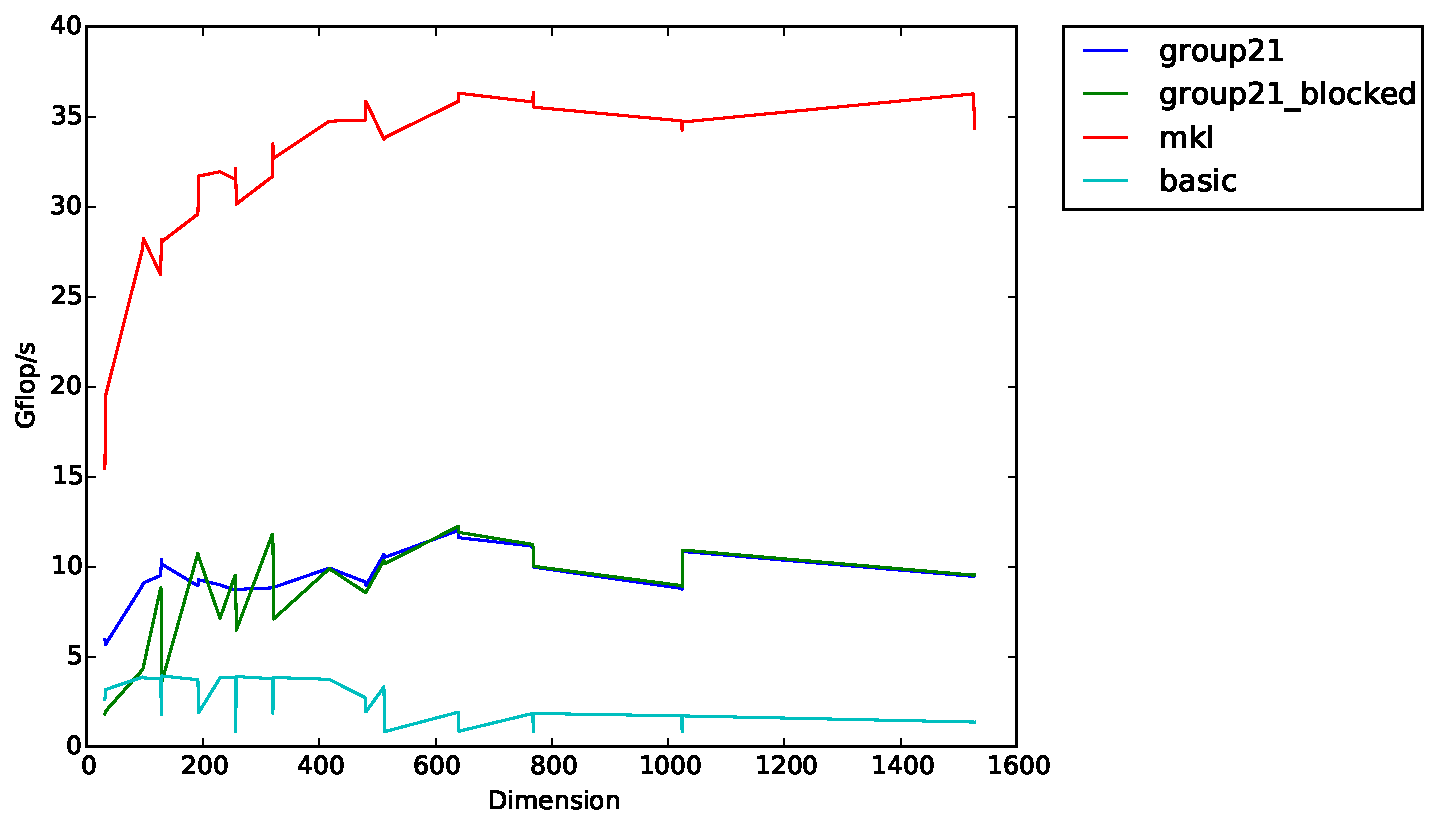
\includegraphics[scale=0.6]{pure_vs_hybrid.pdf}
\caption{Performance comparison: final implementation (hybrid) vs only blocking}
\end{figure}

The compiler flags play a major part in improving the DGEMM routine performance. The flags used in the final implementation are \texttt{-O3 -fast -funroll-loops -ipo -xCORE-AVX2 -no-prec-div -ansi-alias -restrict}. The makefile used is $\texttt{Makefile.in.icc}$. The design decisions of each compiler flag is described in Section \ref{sec:comp_flags}.

\begin{figure}[H]
\centering
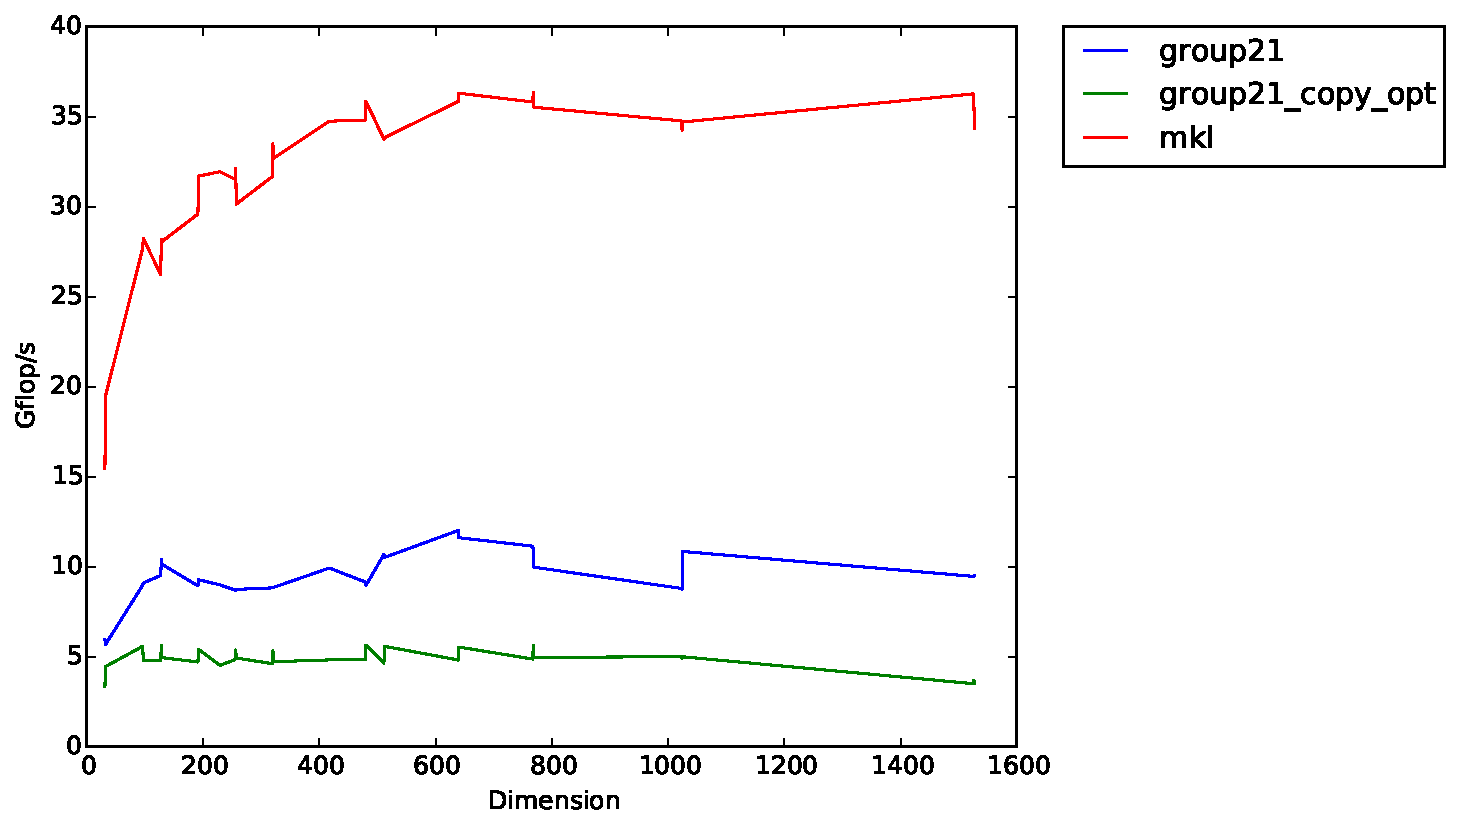
\includegraphics[scale=0.6]{growth_to_stage1.pdf}
\caption{Performance comparison: final implementation vs stage 1 implementation}
\end{figure}

\section{Design Decisions}
\subsection{Compiler Flags}\label{sec:comp_flags}

The final implementation uses the flags, \texttt{-O3 -fast -funroll-loops -ipo -xCORE-AVX2 -axCORE-AVX2 -no-prec-div -ansi-alias -restrict -opt-prefetch}.
\subsubsection{Optimization Level 3}
O3 optimization performs aggressive loop transformations such as Fusion, Block-Unroll-and-Jam, and collapsing IF statements. According to the Intel Developer zone, \cite{stepbystep} O3 is recommended for for applications that have loops that heavily use floating-point calculations and process large data sets.

\subsubsection{Unrolling loops}
The core matrix multiplication kernel performs a dot product with a stride of 1. This behavior is ideal for loop unrolling and is turned on by adding \texttt{-funroll-loops}. Results from manually unrolling loops are described in Section \ref{sec:prev_unroll}.

\subsubsection{Interprocedural Optimization}
The compiler flag \texttt{-ipo} turns on interprocedural optimization to improve performance of the program by letting the compiler analyze the entire program. \cite{ipo}

\subsubsection{Processor Specification}
The processor dispatch option \texttt{-axCORE-AVX2} enables the program to choose the most suitable code path for the Intel Xeon E5-2620 v3 processor. The \texttt{-xCORE-AVX2} flag enables processor specific code generation. \cite{comp_opt}


\subsubsection{Accuracy and Precise Division}
Using the \texttt{-no-prec-div} flag gives slightly less accurate results than full IEEE division. Compiler converts floating point division operations to multiplication by a reciprocal, improving multiplication performance. We also use the \texttt{-fast} flag which may result in slight reduction of accuracy but improvement in performance. 

\subsubsection{Aliasing}

Copy optimization on $A$ in the small matrix case and aligned dynamic memory allocation in the blocked case guarantees that no two pointers in a function point to the same memory location. By using the \texttt{-restrict} flag, we can tell the compiler to prevent alias checking during runtime. \cite{opt} We also use the \texttt{-ansi-alias} flag to tell the compiler that the program adheres to ISO C Standard aliasability rules. Experimentation results are described in \ref{sec:prev_restrict}

\subsubsection{Prefetching}


\subsection{Copy Optimization}\label{sec:copy_opt}
Consider the equation of an element of $C$,

\begin{equation}
	C_{ij} = \sum_k A_{ik} B_{kj}
\end{equation}

In the naive implementation, the innermost loop walks over one of the matrices with stride not equal to 1. In a matrix with size $2^N$, and using column-major storage, the addresses of the elements in a row are  separated by powers of 2. Since the L1 cache is direct-mapped, we run into large number of cache misses. \\


To prevent this behavior, we can switch the storage of $A$ from column-major to row-major. This also improves multiplication for all matrix sizes since the innermost loop has stride 1. The experimentation results for copy optimization are described in Section \ref{sec:prev_copy}.

\subsection{Padded Blocking}\label{sec:block}
In \texttt{dgemm\_blocked.c} and our initial matrix multiplication attempt, (Section \ref{sec:prev_block}), we have extra logic to handle cases where the block size may not be square. Removing this additional logic can improve performance of multiplication since there is less branching logic for blocking. In the setup phase, we allocate matrices padded to the block sizes. Since the padding is done with zeros, the result of the final multiplication is unchanged. Refer to the \texttt{dgemm\_group21.c:padded\_transpose} function for the implementation of padding. \\

Furthermore, the block size was picked to ensure that the blocks of $A$ and $B$ both fit in the L1 cache of the processor. The L1 cache of the Intel Xeon E5-2620 v3 has the ability to hold 6 x 32KB data. Then, to fit both $A$ and $B$ blocks, we have to satisfy, 2 * \texttt{BLOCK\_SIZE} * \texttt{BLOCK\_SIZE} * 8B = 192KB. Then block sizes $< 100$ would fit in the L1 cache. Our experiments in Section \ref{sec:prev_block} guided us to pick 32 as the \texttt{BLOCK\_SIZE}.


\subsection{Memory Alignment}\label{sec:align}
To increase the efficient of data loads (in the case of reading elements of $A$ and $B$) and stores (writing back to $C$), it is useful to force the compiler to make the dynamically allocated memory blocks aligned on specific byte boundaries. \cite{vectorization} In the blocked approach of the final implementation, we reallocate memory for $A, B,$ and $C$ aligned to 64 byte boundaries using \texttt{\_mm\_malloc}. To tell the compiler about the alignment of the matrices, in the innermost loop of the multiplication of a block, we use the clause \texttt{\_\_assume\_aligned}. \cite{vectorization}

\section{Unsuccessful Optimization Attempts}
\subsection{Fitting to L2 cache}
The L2 cache of the Xeon processor can hold 6 x 256KB data. Then, we should be able to increase the block size by $\sqrt(8)$ and notice an improvement in performance. Our experiments showed that the performance decreases when we increase the \texttt{BLOCK\_SIZE} to 128.  

\begin{figure}[H]
\centering
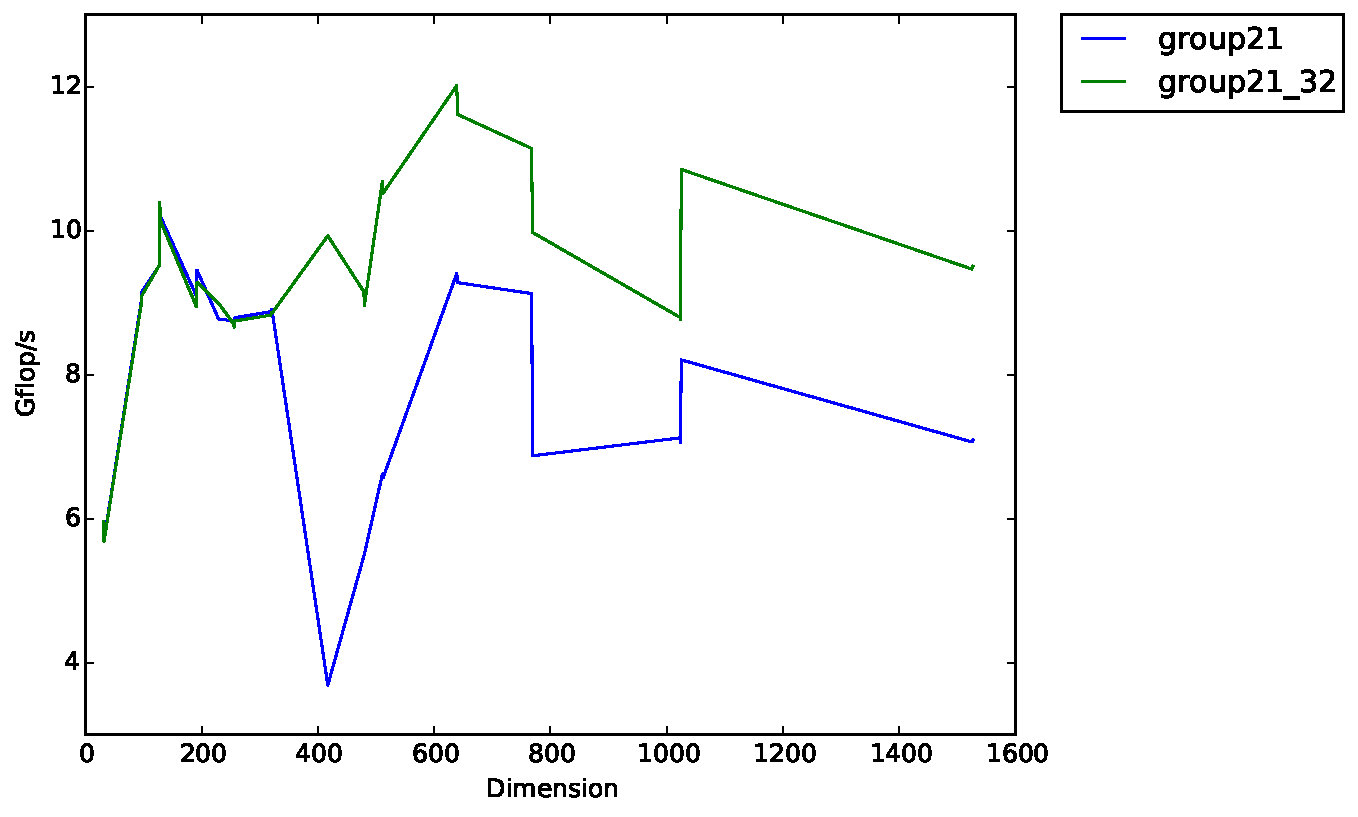
\includegraphics[scale=0.6]{128_32.pdf}
\caption{Performance comparison: \texttt{BLOCK\_SIZE} 128 vs 32}
\end{figure}

We believe that this performance decrease occurs due to blocks not fitting in the L1 cache.

\subsection{Blocking approach in smaller matrices}
We adopted a hybrid multiplication approach since on smaller matrices, the blocked approach performs worse than tight loops with copy optimization. 

\begin{figure}[H]
\centering
\label{blocked_spiky}
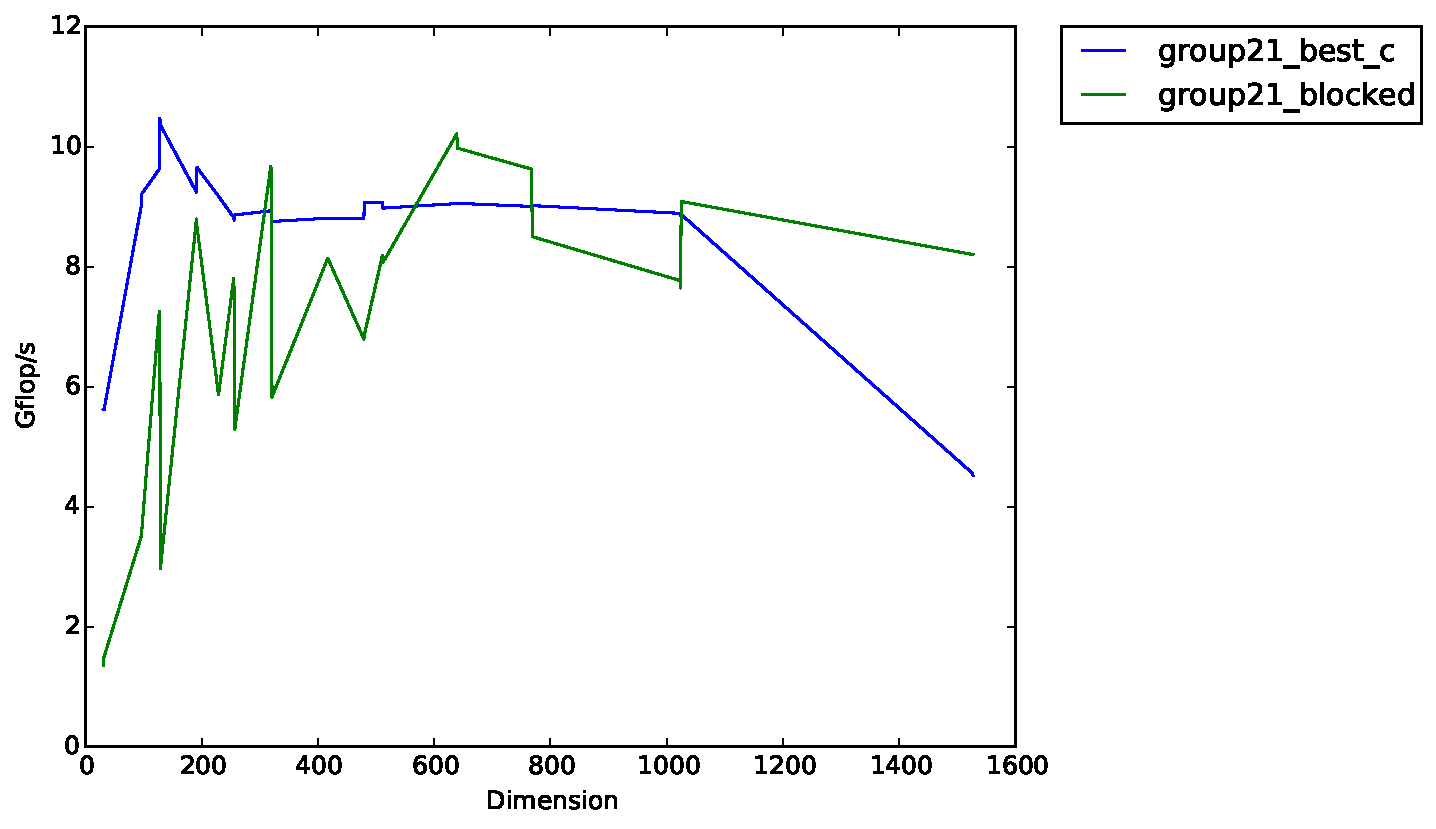
\includegraphics[scale=0.6]{blocked_small.pdf}
\caption{Performance comparison: Tight loops with copy optimization vs blocked approach}
\end{figure}

We believe that on smaller matrix sizes, the overhead of aligned memory reallocation and blocking reduces performance compared to tight loops with copy optimization. Also, in figure \ref{blocked_spiky}, we see significant drops in performances in matrix sizes 129, 229, 257 and 321. The matrices with leading dimension $< 300$ would fit in the L2 cache and the blocking approach should perform as well as the tight loops. But the zig zag pattern we see  show, on average, lower performance than the tight loops approach.  We were unable to diagnose the cause of the zig-zag pattern in the performance. 

\section{Optimization Experiments}
\subsection{Block Multiplication with Multiple Block Sizes} \label{sec:prev_block}
\subsubsection{Approach}
Working off of \texttt{dgemm\_blocked.c}, we tried different block sizes to examine the performance changes. 
\subsubsection{Results}
Figure \ref{pow_2_blocks} shows the performance of different approaches with various block sizes. (block sizes are a multiple of 2). The performance gain for varying block sizes is not immense but a block size of 64 performs better than other block sizes. \\

\begin{figure}[H]
    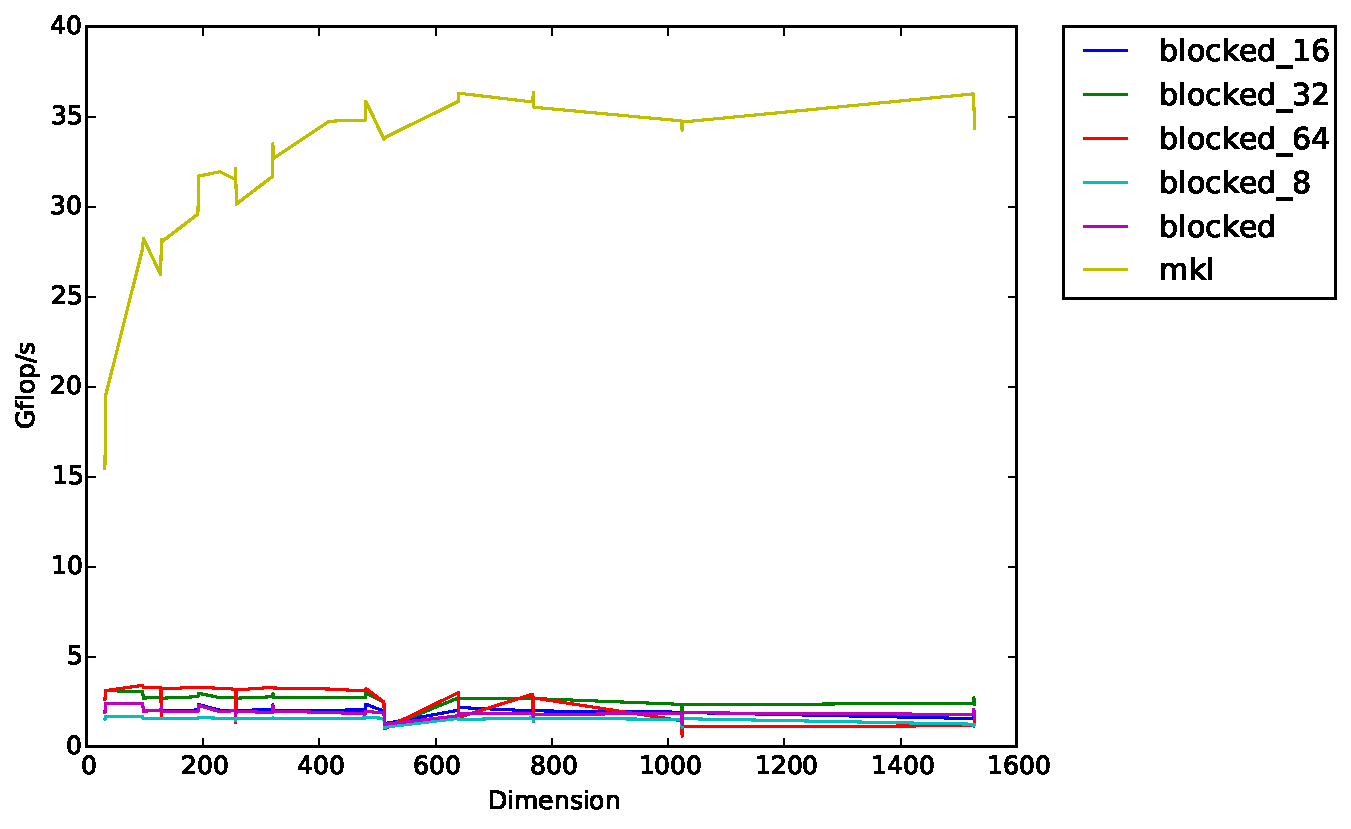
\includegraphics[width=0.9\textwidth]{timing_block_size_changes.pdf}
    \caption{Block size variation}
    \label{pow_2_blocks}
\end{figure} 

In addition, we attempted block sizes that are not a multiple of 2. Figure \ref{odd_blocks} is the comparison of the performance against a block size of 64.\\
\begin{figure}[H]
    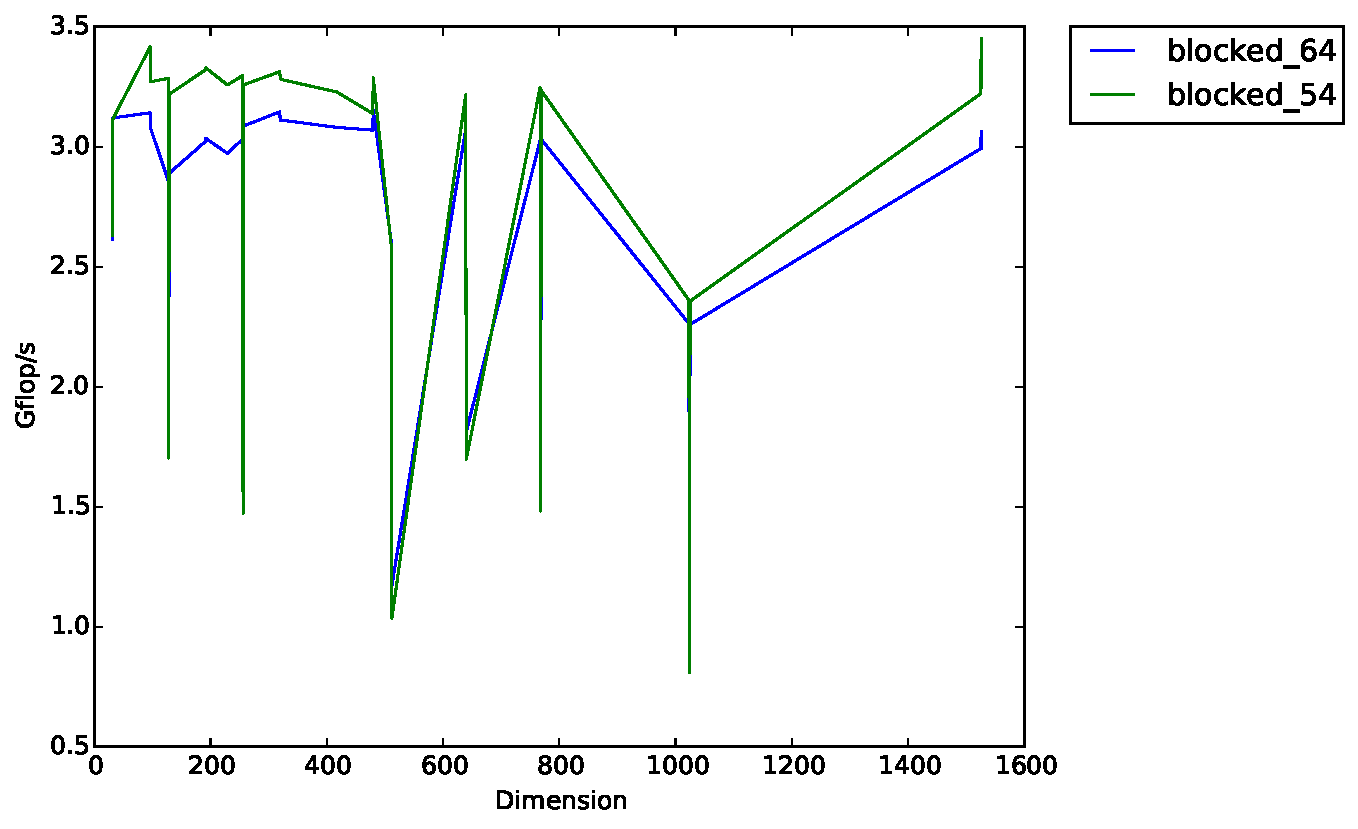
\includegraphics[width=0.9\textwidth]{timing_54_64.pdf}
    \caption{Block size variation}
    \label{odd_blocks}
\end{figure} 


\subsection{Block Multiplication with Manual Loop Unrolling} \label{sec:prev_unroll}
\subsubsection{Approach}
In this approach, we manually unrolled 4 computations in the inner most loop of the matrix multiplication of a block. 
\subsubsection{Results}
Figure \ref{unrolled_vs_regular} compares the performance of the unrolled blocked version against the vanilla blocked approach. The unrolled versions clearly perform better than the original blocked approach but not by much. 
\begin{figure}[H]
    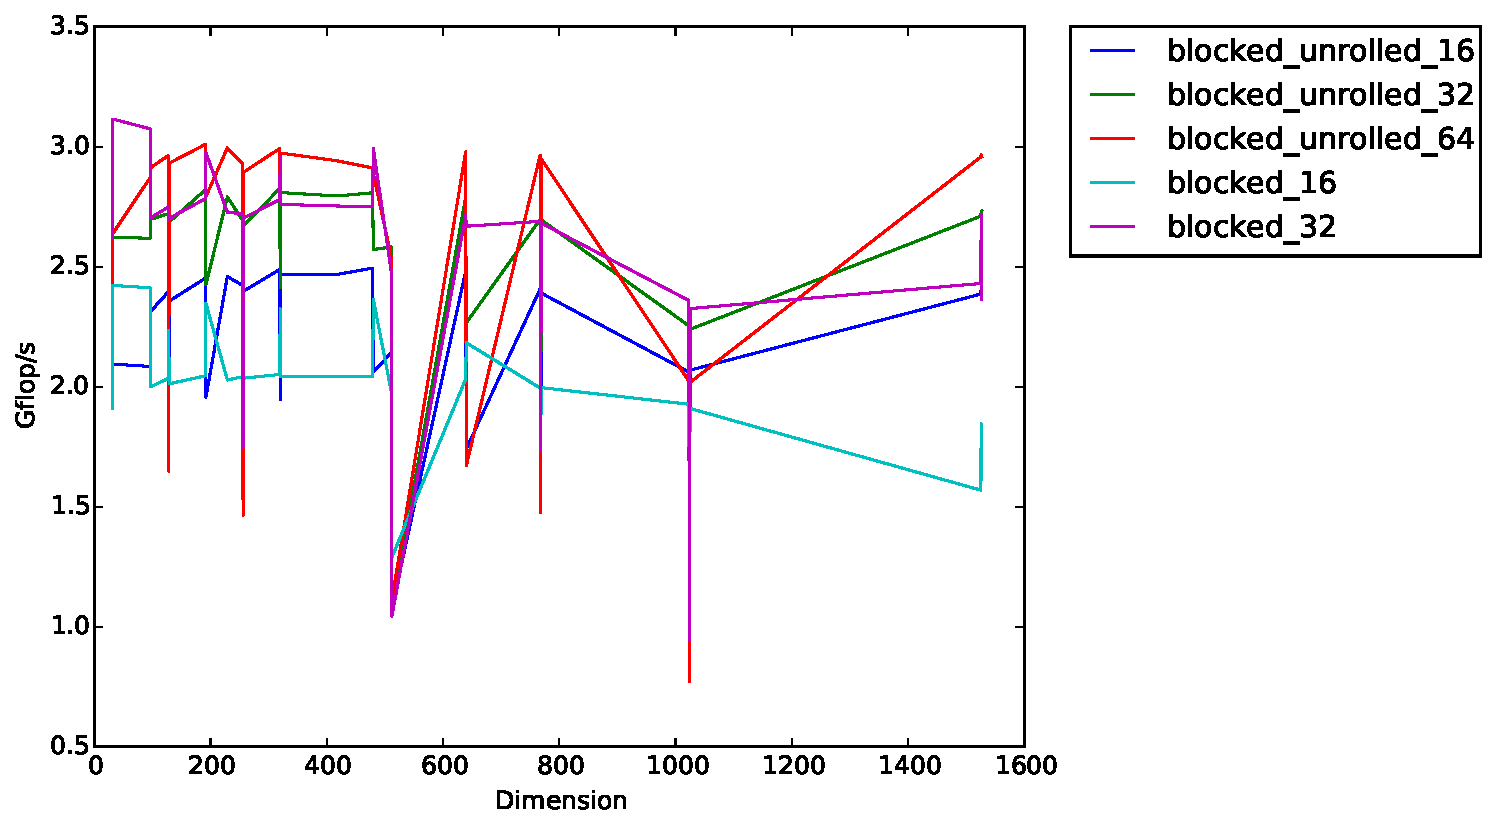
\includegraphics[width=0.9\textwidth]{timing_unrolled_vs_nonunrolled.pdf}
    \caption{Unrolled blocks vs regular blocks}
    \label{unrolled_vs_regular}
\end{figure} 

\subsection{Compiler Optimization Flags}
\subsubsection{Approach}
Using the blocked approach as a baseline, we examine the effect of various compiler flags on the multiplication.
\subsubsection{Results}
Figure \ref{all_optimized_blocked} shows the performance of blocked multiplication with the flags, \texttt{-O3 -march=native -funroll-loops}.
\begin{figure}[H]
    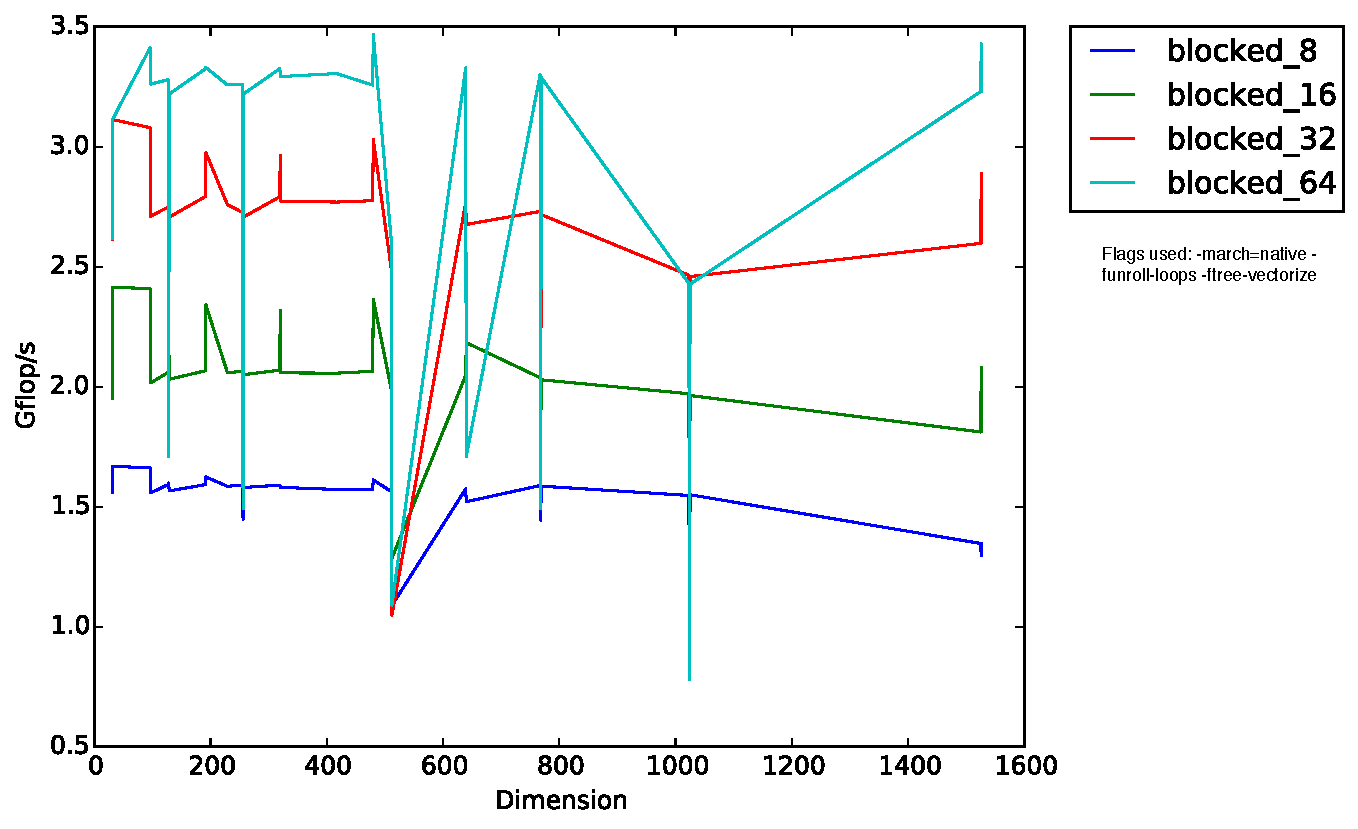
\includegraphics[width=0.9\textwidth]{timing_flags_blocked.pdf}
    \caption{Compiler flags \texttt{-O3 -march=native -funroll-loops}}
    \label{all_optimized_blocked}
\end{figure} 

Figure \ref{funroll_vanilla} shows the performance of blocked multiplication with the flags, \texttt{-O3 -funroll-loops} vs just \texttt{-O3}. It appears that merely having the \texttt{-O3} flag performs as well as having loops unrolled. 
\begin{figure}[H]
    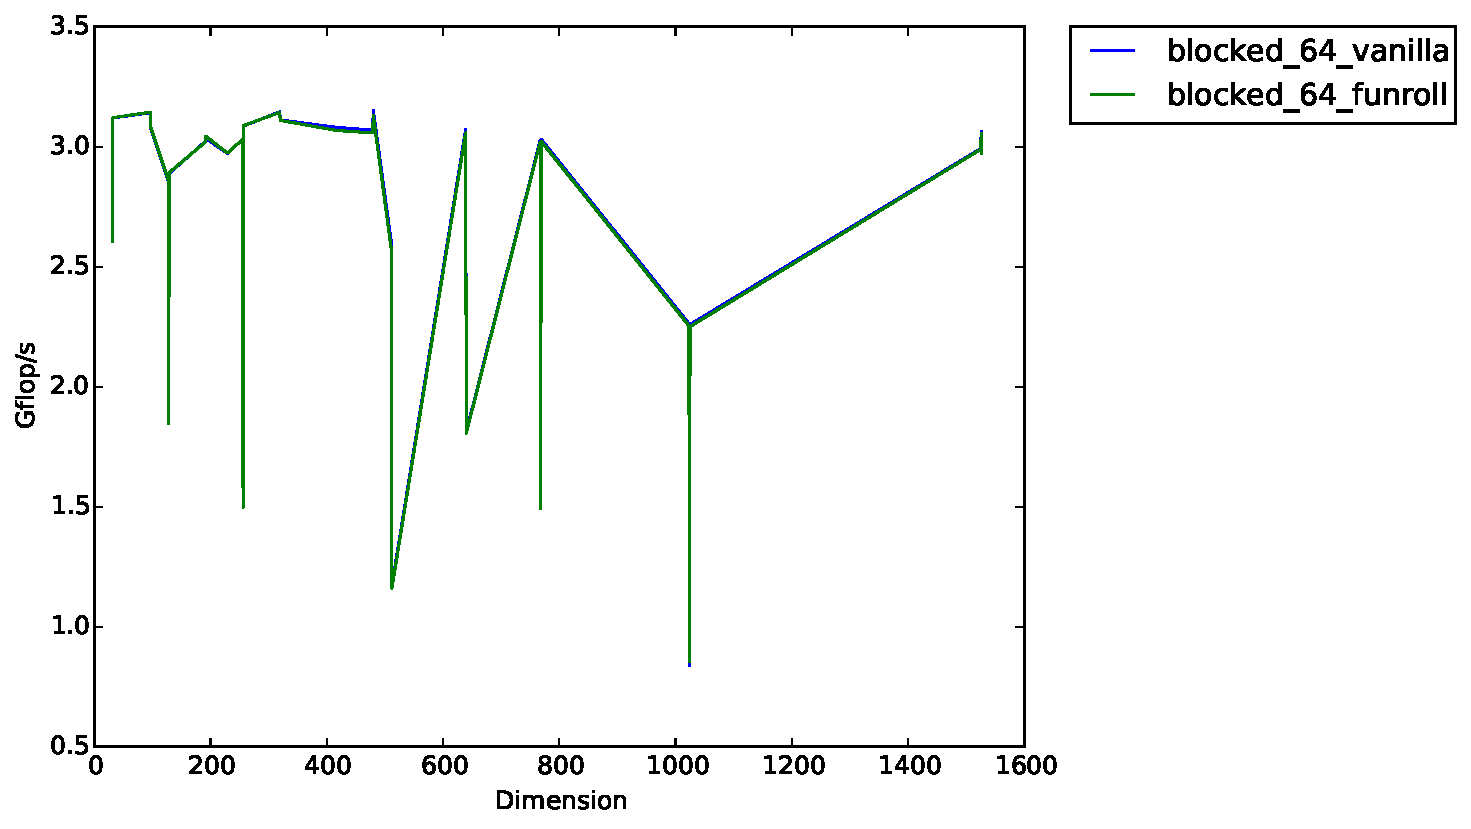
\includegraphics[width=0.9\textwidth]{timing_funroll_vanilla.pdf}
    \caption{Compiler flags \texttt{-O3 -funroll-loops}}
    \label{funroll_vanilla}
\end{figure} 


\subsection{Loop reordering}
\subsubsection{Approach}
The current block multiplication in the innermost loop does not have unit stride with $i, j, k$ loop ordering. 
\subsubsection{Results}

\begin{figure}[H]
    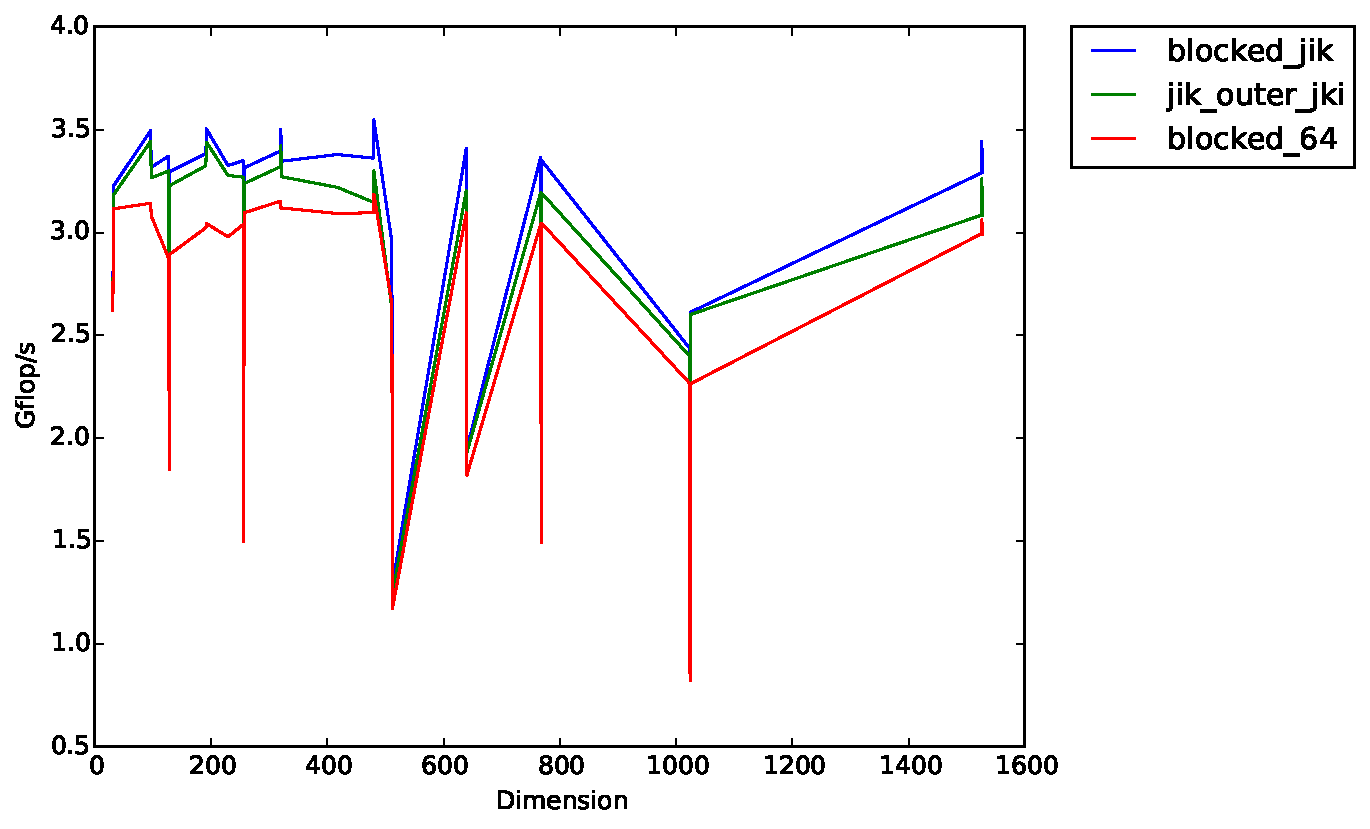
\includegraphics[width=0.9\textwidth]{timing_loop_reorder_fast.pdf}
    \caption{Loop reordering \texttt{ijk} vs \texttt{jik} vs \texttt{jik} and outer loop \texttt{jki}}
    \label{basic_copy_opt}
\end{figure} 

\subsection{Copy Optimization} \label{sec:prev_copy}
\subsubsection{Approach}
In the basic version of dgemm, we see drops near matrix sizes that are a multiple of 2. This is caused by conflict misses due to associative caches. To prevent this, we attempted a copy optimization over the basic dgemm implementation.
\subsubsection{Results}
There is a clear improvement in performance and the conflict misses are converted to gains in performance as seen in Figure \ref{basic_copy_opt}. Copy optimization is clearly a step in the right direction.
\begin{figure}[H]
    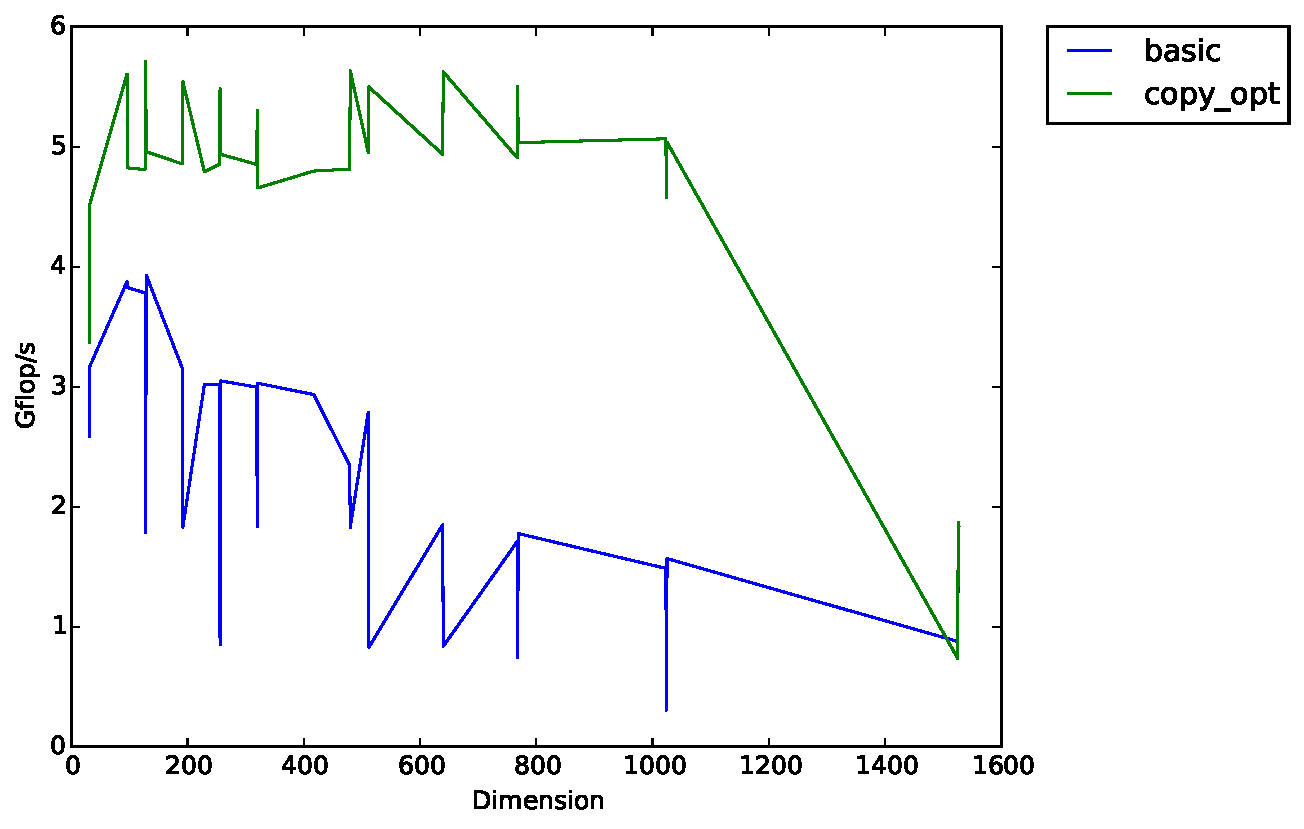
\includegraphics[width=0.9\textwidth]{timing_basic_vs_copy_opt.pdf}
    \caption{Basic DGEMM vs DGEMM with Copy Optimization}
    \label{basic_copy_opt}
\end{figure} 
\subsection{Compiler flags on Copy Optimization}
\subsubsection{Approach}
We use \texttt{-03} and \texttt{-02} optimization flags when we compile the copy optimization code.
\subsubsection{result}
\texttt{-02} optimizer is performing better than \texttt{-03}  especially when the size of the matrix grows larger.
\begin{figure}[H]
    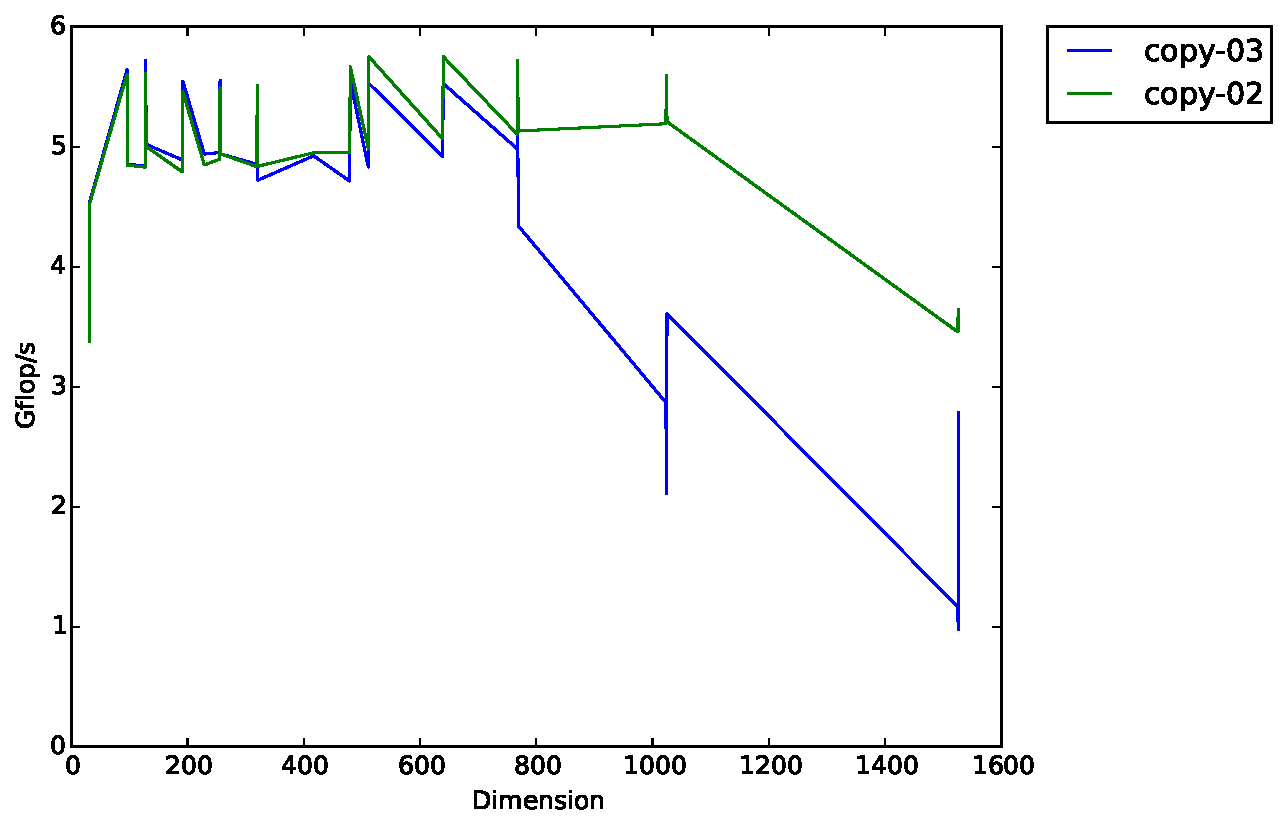
\includegraphics[width=0.9\textwidth]{timing_flag0203_copy.pdf}
    \caption{-03 vx -02 on Copy Optimization}
    \label{0203}
\end{figure}
 

\subsection{Restrict Keyword} \label{sec:prev_restrict}

\subsubsection{Approach}
Telling the compiler that our matrix pointers will not be aliasing is another approach suggested on the writeup. 
\subsubsection{Results}

Figure \ref{basic_restrict} shows the performance difference between the basic DGEMM implementation and the DGEMM implementation with the \texttt{restrict keyword}. \texttt{restrict} keyword provides good performance benefits. There is a caveat here since we assumed that the pointer \texttt{A} and \texttt{B} passed to \texttt{square\_dgemm} will not alias. 

\begin{figure}[H]
    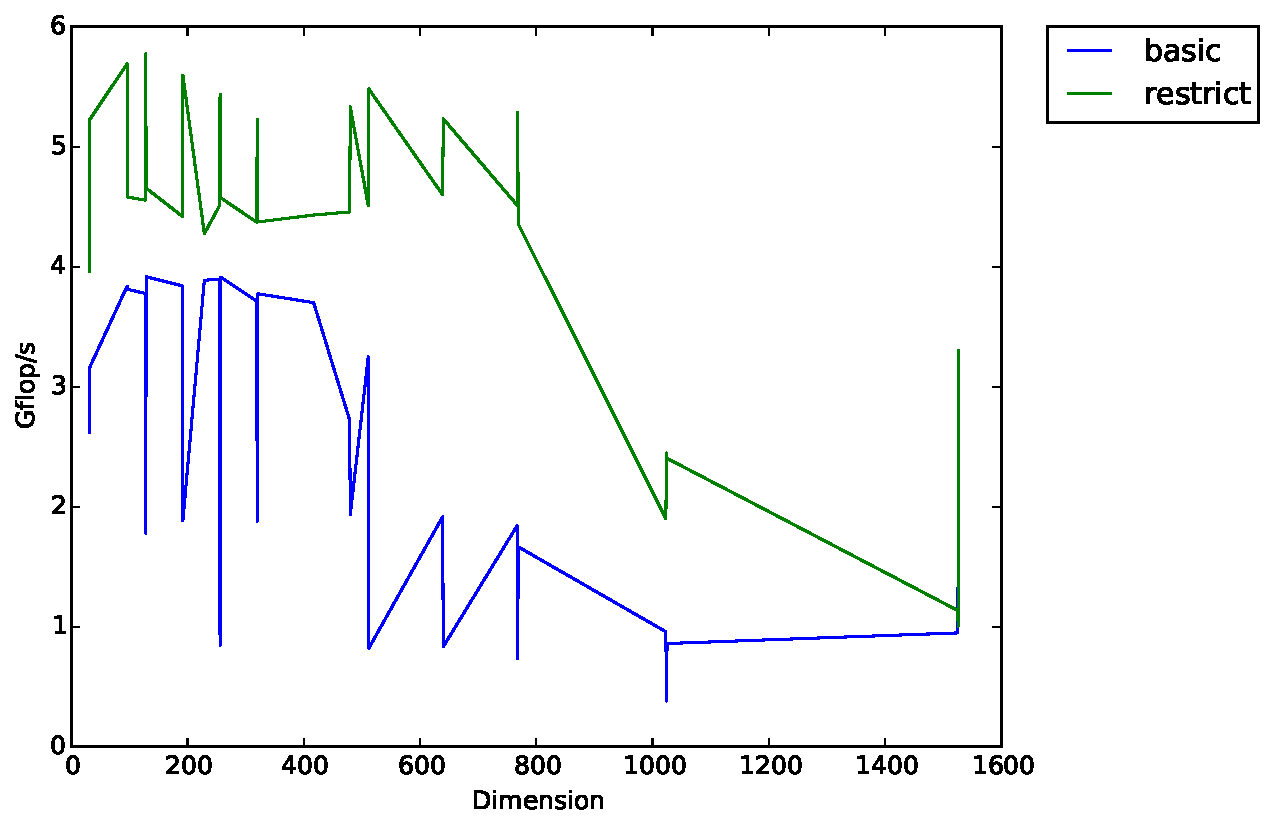
\includegraphics[width=0.9\textwidth]{timing_basic_vs_restrict.pdf}
    \caption{Basic DGEMM vs DGEMM with \texttt{restrict} keyword}
    \label{basic_restrict}
\end{figure} 

To eliminate the aliasing assumption, we intended to couple the \texttt{restrict} keyword and copy optimization to provide a stronger guarantee of not aliasing. The result as shown in figure \ref{restrict_copy_opt} shows that the performance decreases. This may be due to incorrect implementation of the restrict keyword in our code. 

\begin{figure}[H]
    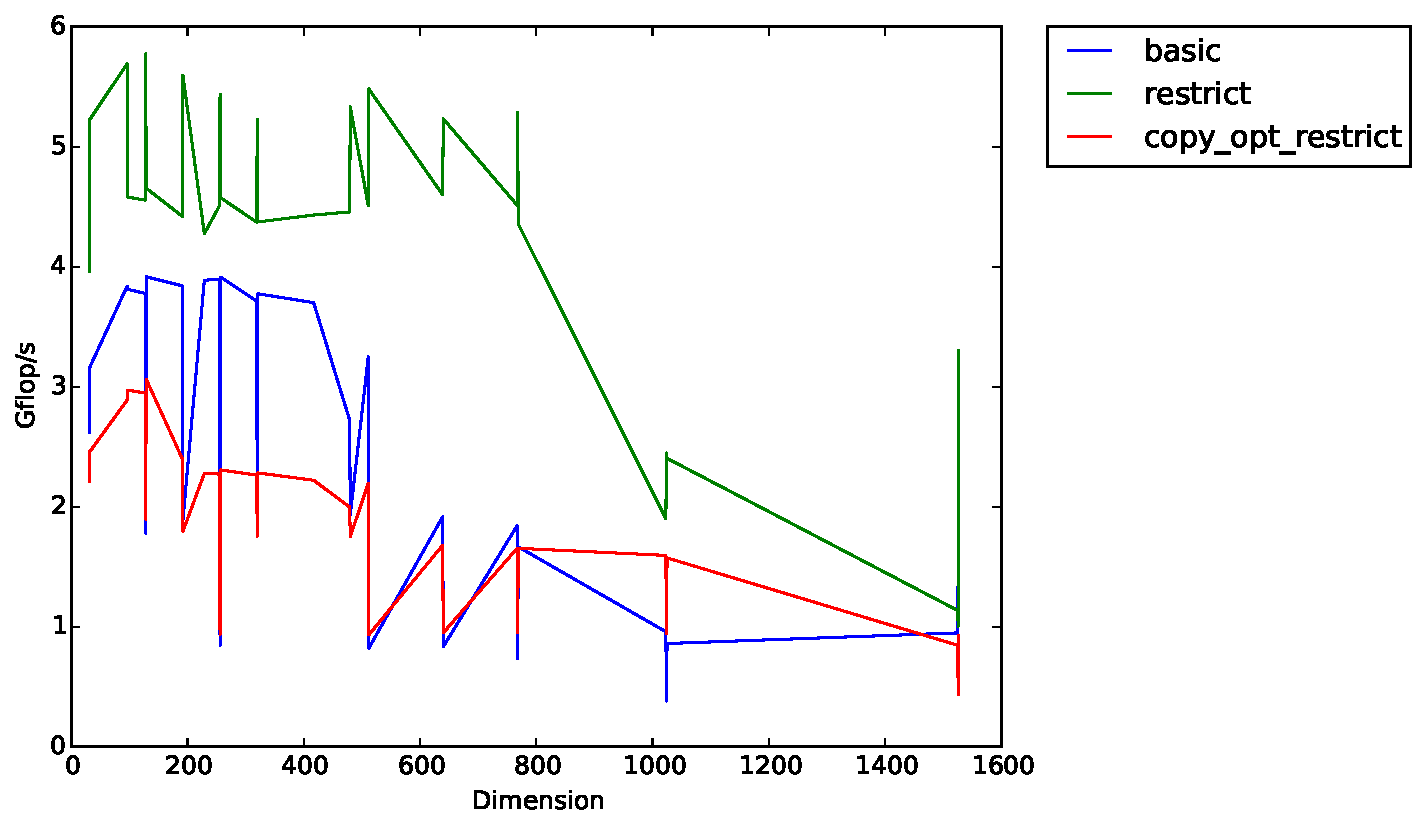
\includegraphics[width=0.9\textwidth]{timing_copy_opt_restrict.pdf}
    \caption{Basic DGEMM vs DGEMM with \texttt{restrict} keyword}
    \label{restrict_copy_opt}
\end{figure} 


\begin{thebibliography}{9}
\bibitem{vectorization} 
Data Alignment to Assist Vectorization. (n.d.). Retrieved September 30, 2015, from \url{https://software.intel.com/en-us/articles/data-alignment-to-assist-vectorization}
 
\bibitem{alignment} 
Memory Management for Optimal Performance on Intel\textsuperscript{\textregistered} Xeon Phi\textsuperscript{\texttrademark} Coprocessor: Alignment and Prefetching. (n.d.). Retrieved September 30, 2015, from \url{https://software.intel.com/en-us/articles/memory-management-for-optimal-performance-on-intel-xeon-phi-coprocessor-alignment-and}

\bibitem{manpages} 
Manpage of ICC. (n.d.). Retrieved September 30, 2015, from \url{http://scv.bu.edu/computation/bladecenter/manpages/icc.html}
 
\bibitem{opt_q} 
Quick-Reference Guide to Optimization with Intel\textsuperscript{\textregistered} Compilers. (n.d.). Retrieved September 30, 2015, from \url{https://software.intel.com/sites/default/files/compiler_qrg12.pdf}

\bibitem{reports}
Getting the Most out of your Intel\textsuperscript{\textregistered} Compiler with the New Optimization Reports. (n.d.). Retrieved September 30, 2015, from \url{https://software.intel.com/en-us/articles/getting-the-most-out-of-your-intel-compiler-with-the-new-optimization-reports}

\bibitem{ipo}
Improving Performance with Interprocedural Optimization. (n.d.). Retrieved September 30, 2015, from \url{https://software.intel.com/en-us/node/590470}

\bibitem{stepbystep}
Step by Step Performance Optimization with Intel\textsuperscript{\textregistered} C Compiler. (n.d.). Retrieved September 30, 2015, from \url{https://software.intel.com/en-us/articles/step-by-step-optimizing-with-intel-c-compiler}

\bibitem{opt}
A Guide to Vectorization with Intel\textsuperscript{\textregistered} C Compilers. (n.d.). Retrieved October 1, 2015, from \url{https://d3f8ykwhia686p.cloudfront.net/1live/intel/CompilerAutovectorizationGuide.pdf}

\bibitem{comp_opt}
Intel\textsuperscript{\textregistered} Compiler Options for Intel\textsuperscript{\textregistered} SSE and Intel\textsuperscript{\textregistered} AVX generation and processor-specific optimizations. (n.d.). Retrieved October 1, 2015, from \url{https://software.intel.com/en-us/articles/performance-tools-for-software-developers-intel-compiler-options-for-sse-gene\\ration-and-processor-specific-optimizations}



\end{thebibliography}

 
 
\end{document}
